\section{Metodología Propuesta}

\subsection{Arquitectura del Sistema}

\begin{figure}[t]
\centering
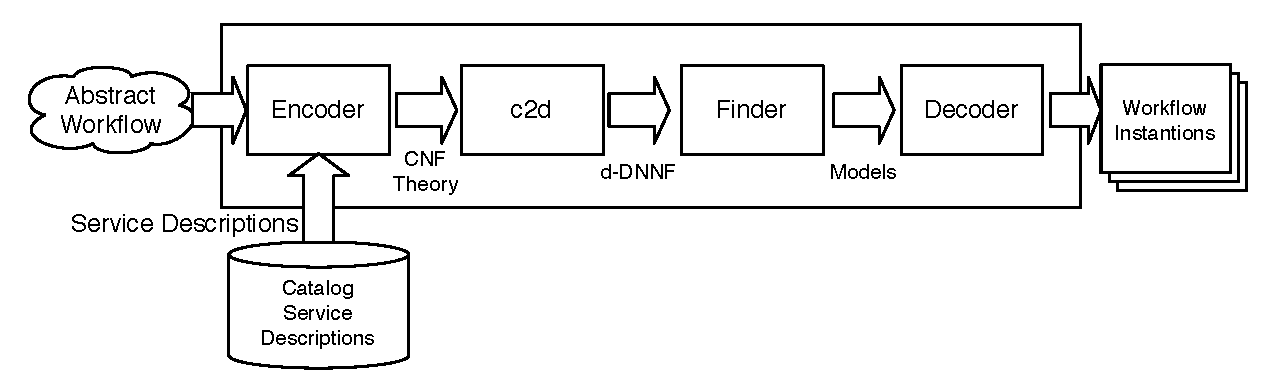
\includegraphics[width=.9\textwidth]{graphics/architecture}
\caption{Arquitectura del Sistema}
\label{fig:architecture}
\end{figure}

Se utiliza una arquitectura comprendida por un catálogo de descripciones de
servicio, el Codificador, el compilador c2d, el Buscador de mejores modelos, y
el Decodificador. La figura~\ref{fig:architecture} muestra la arquitectura global del sistema.
En esta infraestructura, una instancia del problema de instanciación de flujos
de trabajo se define como un flujo abstracto representado por una consulta
conjuntiva sobre servicios abstractos que es dada como entrada junto con un
conjunto de servicios concretos definidos por vistas de servicios abstractos.

El catálogo se pobla con descripciones de servicios abstractos y concretos; cada
servicio es descrito en términos de atributos de entrada y salida y anotado con
un valor real que representa la utilidad QoS del servicio. La descripción de los
servicios concretos, que son definidos como vistas de los servicios abstractos,
puede ser generada de manera semiautomática o automática usando herramientas
tales como el sistema DEIMOS \cite{AmbiteISWC09}.

Una instancia de entrada de WIP es codificada como una teoría CNF cuyos modelos
corresponden a las intanciaciones del flujo de trabajo por el Codificador. El
compilador c2d, un componente \emph{off-the-shelf}, compila la fórmula CNF a
d-DNNF. El Codificador traduce las instancias WIP en teorías CNF que luego son
convertidas en d-DNNF usando c2d. El Buscador computa un mejor modelo dados los
parámetros QoS en tiempo lineal en el tamaño del d-DNNF resultante. Es
importante remarcar que el proceso de compilación necesita ser realizado sólo
una vez ya que no depende del valor de los parámetros QoS. Así, incluso si la
compilación resulta ser costosa en términos de tiempo, este costo puede ser
amortizado dado que el d-DNNF resultante puede ser usado para conseguir mejores
instanciaciones con respecto a múltiples valores de los parámetros QoS.
Finalmente, el Decodificador traduce el mejor modelo retornado por el Buscador
a una instanciación de flujo de trabajo que resuelve el WIP.

Dado un CNF que codifica un WIP, su d-DNNF es una representación compacta de
todas las instanciaciones del flujo de trabajo. Es decir, uno puede generar de
una manera libre de \emph{backtracking} todas las instanciaciones del flujo de
trabajo. Si el usuario está interesado en una mejor instanciación dados
parámetros de QoS, entonces esta se puede computar en tiempo lineal en el tamaño
del d-DNNF. Si el usuario está interesado en todas las mejores instanciaciones,
estas pueden ser computadas en tiempo lineal en su número. Finalmente, si el
usuario está interesado en todas las instanciaciones, estas también pueden ser
computadas en tiempo lineal en su número. En los últimos dos casos, si ese
número es exponencial (en el tamaño de la entrada), la enumeración de las
instanciaciones también lo es pero esta complejidad es intrínsica al problema y
por lo tanto no puede ser evitada.

